\documentclass[tikz,border=2pt]{standalone}
\renewcommand{\familydefault}{\sfdefault}
\usetikzlibrary{arrows.meta,calc,positioning}
\tikzset{every picture/.style={line width=1pt, >=Stealth},
         hl/.style={fill=black, fill opacity=0.12, text opacity=1}}
\begin{document}
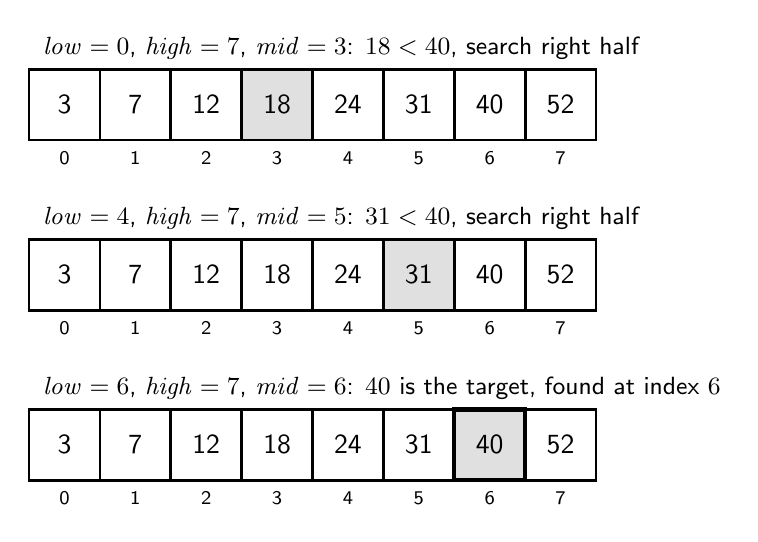
\begin{tikzpicture}[x=0.9cm, y=0.9cm, cell/.style={draw, minimum size=0.9cm},
    found/.style={hl, line width=1.6pt}]
  % \row{y}{value/style, ...}: one array, with each index below its cell
  \newcommand{\row}[2]{\foreach \v/\s [count=\i from 0] in {#2} {
    \node[cell, \s] at (\i, #1) {\v};
    \node[font=\scriptsize] at (\i, #1 - 0.75) {\i};
  }}
  \node[right, font=\small] at (-0.45, -0.0 + 0.8) {$\mathit{low} = 0$, $\mathit{high} = 7$, $\mathit{mid} = 3$: $18 < 40$, search right half};
  \row{-0.0}{3/,7/,12/,18/hl,24/,31/,40/,52/}
  \node[right, font=\small] at (-0.45, -2.4 + 0.8) {$\mathit{low} = 4$, $\mathit{high} = 7$, $\mathit{mid} = 5$: $31 < 40$, search right half};
  \row{-2.4}{3/,7/,12/,18/,24/,31/hl,40/,52/}
  \node[right, font=\small] at (-0.45, -4.8 + 0.8) {$\mathit{low} = 6$, $\mathit{high} = 7$, $\mathit{mid} = 6$: $40$ is the target, found at index $6$};
  \row{-4.8}{3/,7/,12/,18/,24/,31/,40/found,52/}
\end{tikzpicture}
\end{document}
